
\section{Funcionamiento del trigger y simulación de pulsos}

Esta sección se basaría principalmente en contar que teníamos problemas con el trigger y contar cómo nos aseguramos de que la RP triggereara bien a través de la medición de la señal serrucho (bastante pava), y la simulación y adquisición de pulsos con la rp.

imagenes tipo

\begin{figure*}[h]
    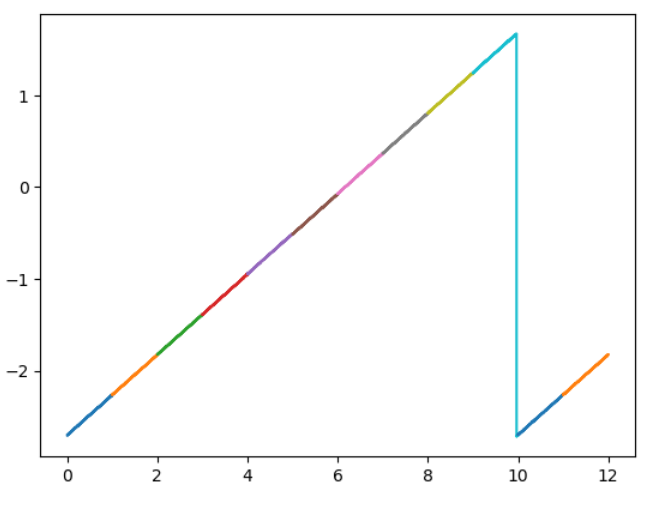
\includegraphics[width=\textwidth]{cap3_tmp2.png}
\end{figure*}

%\begin{figure*}[h]
%    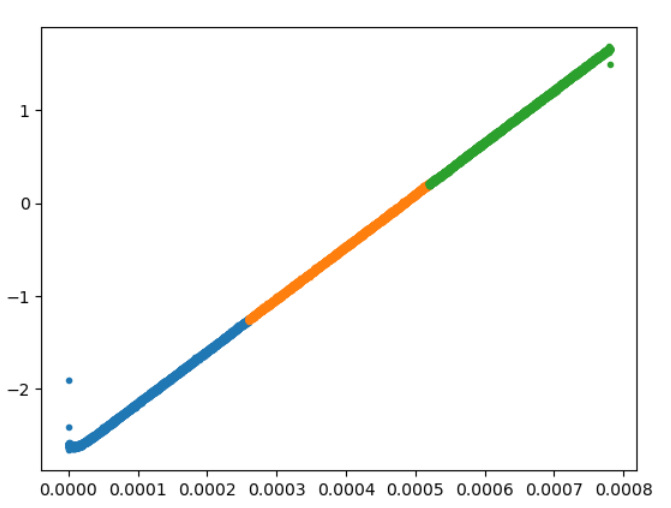
\includegraphics{cap3_tmp1.png}
%\end{figure*}

\section{Caracterización del PMT}

acá pienso poner el análisis que hice para ver que tipo de pulsos había en el PMT, graficos como estos (que hice similares para 5 sampling rate distintos de la RP): \\
\ref{fig:a} \\
\ref{fig:b} \\
\ref{fig:c} \\
\ref{fig:d} \\
\ref{fig:e} \\
\ref{fig:h} \\

todo me parece muy boludo la verdad, lo único interesante es la autocorrelación...

\begin{figure*}[h]
    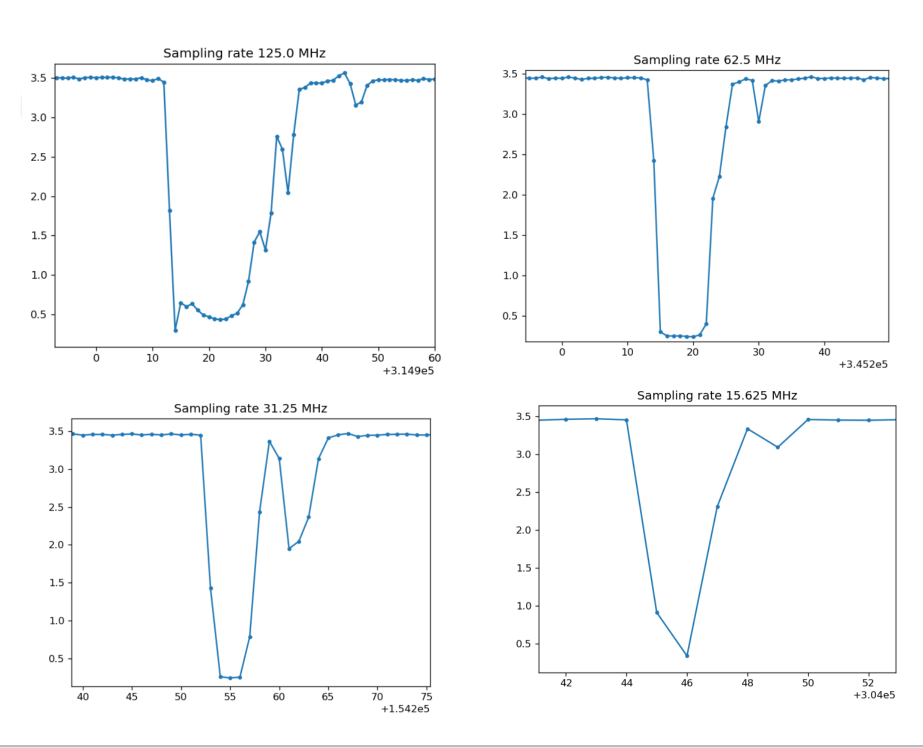
\includegraphics[width=\textwidth]{cap3_tmp3.png}
    \label{fig:a}
\end{figure*}

\begin{figure*}[h]
    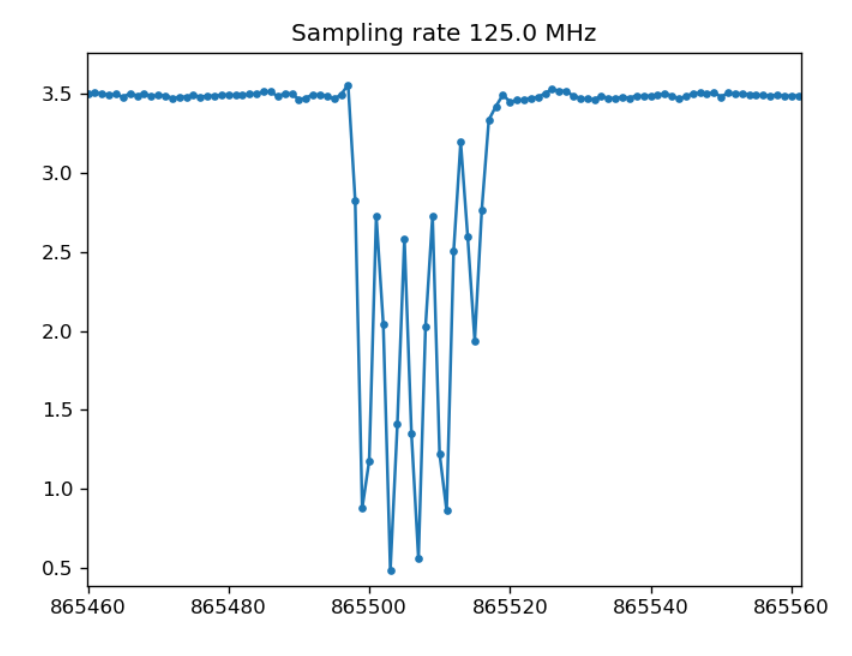
\includegraphics[width=\textwidth]{cap3_tmp4.png}
    \caption{picos raros que aparecen a veces}
    \label{fig:b}
\end{figure*}

\begin{figure*}[h]
    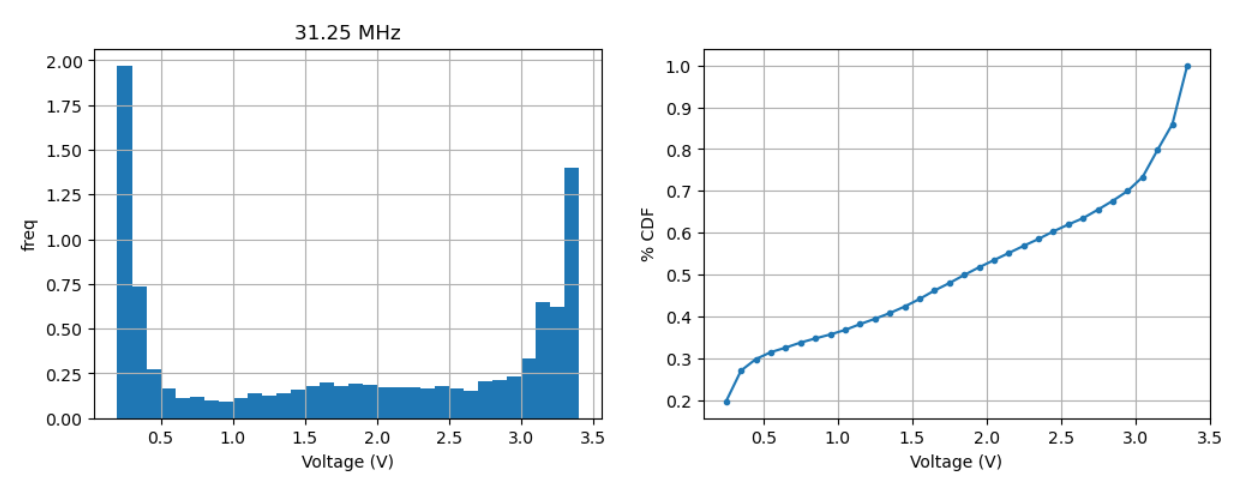
\includegraphics[width=\textwidth]{cap3_tmp5.png}
    \caption{histograma de la altura de los picos}
    \label{fig:c}
\end{figure*}

\begin{figure*}[h]
    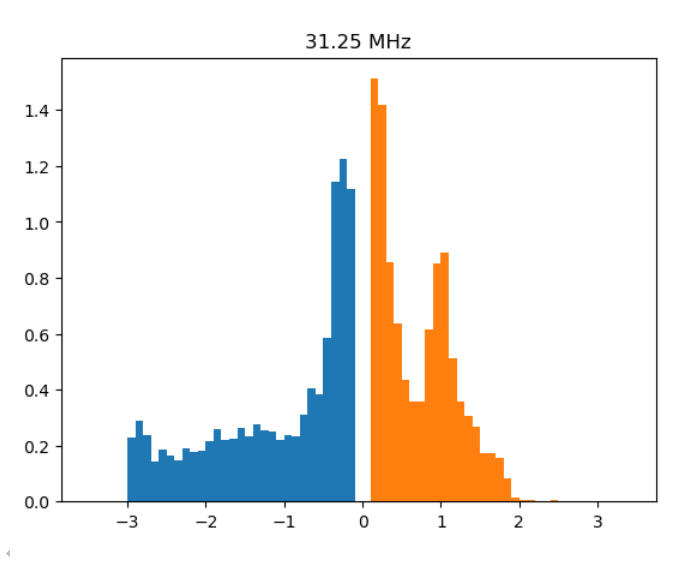
\includegraphics[width=\textwidth]{cap3_tmp6.png}
    \caption{distr de la derivada. Lo puse porq la uso para contar pero no tiene mucha gracia}
    \label{fig:d}
\end{figure*}

\begin{figure*}[h]
    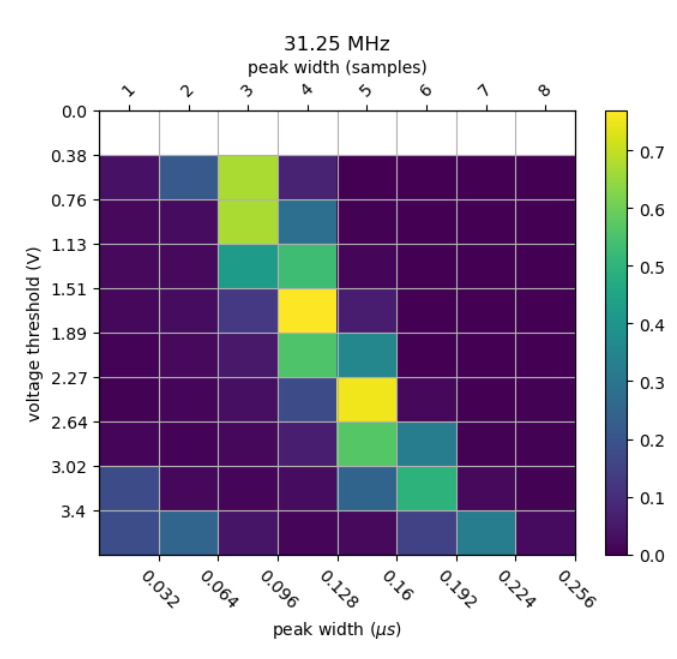
\includegraphics[width=\textwidth]{cap3_tmp7.png}
    \caption{distribución de la cantidad de samples que quedan por debajo/arriba de un threshold en funcion de la altura de ese threshold. Tengo uno para cada samplig rate}
    \label{fig:e}
\end{figure*}

\begin{figure*}[h]
    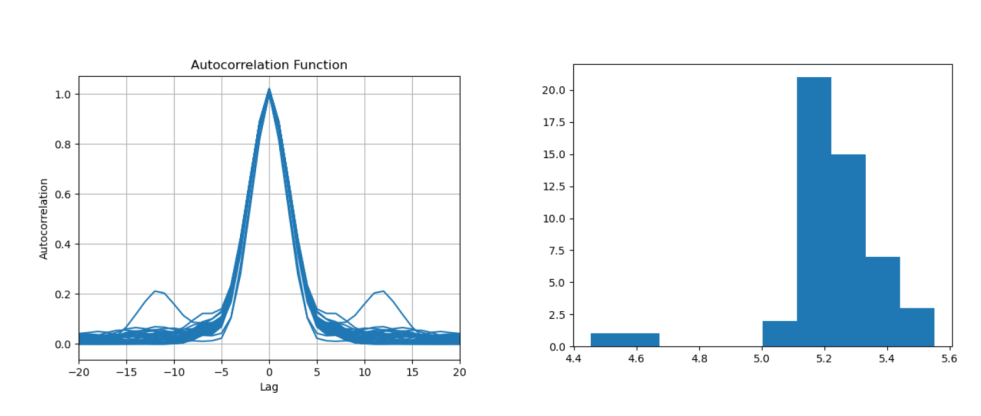
\includegraphics[width=\textwidth]{cap3_tmp8.png}
    \caption{autocorrelacion de los picos. Tmb tengo un fit gausiano para ver el ancho.}
    \label{fig:h}
\end{figure*}

\section{Conteo de fotones}

Acá pensaba poner 
\begin{enumerate}
    \item lo que daría la distribución de distancia entre fotones si la prob de medir un foton es uniforme
    \item mostraría lo que da la distribución para distintos métodos de conteo de picos para los datos que medí yo.
\end{enumerate}

\section{validación patrón}

Acá va:

\begin{enumerate}
    \item comparación de medición de espectro de excitación y absorción de la rhodamina medido con felix y con nuestro refurbishment
    \item comparación del tiempo de vida de nuestras mediciones con las de juan u algún otro paper.
\end{enumerate}

%tengo:
%
%\begin{itemize}
%    \item simulación de pulsos con la rp conectada a si misma
%    \item medición de ventanas distintas trigger
%    \item simulación de picos y lo que debería dar conteo correcto
%    \item conteo de picos con distintas técnicas
%    \item imágenes de los picos a varias SR
%    \item altura de picos en func de la altura
%    \item ancho picos en funcion de la altura Y SR
%    \item autocorrelación
%\end{itemize}